\subsection{Principes et état de l’art des systèmes de séparation d’étages}
\label{sec:etat_art_separation}

La littérature technique et scientifique distingue les dispositifs de séparation d’étages selon deux grands critères : le mode
d’activation et la nature des efforts mobilisés pour obtenir une séparation fiable entre les segments du lanceur.

\subsubsection{Modes de séparation d’étages}

\subsubsubsection{Pyrotechnique}

Les dispositifs pyrotechniques représentent une des méthodes les plus répandues dans l’industrie spatiale pour séparer des
étages. Ils reposent sur l’utilisation de charges explosives intégrées dans des éléments de fixation (ex. boulons explosifs ou
frangible nuts) qui, lorsqu’elles sont activées, rompent instantanément la liaison structurelle entre deux éléments
\cite{Pyrotechnic_StageSeparation}\cite{Pyrotechnic_Fastener}.\\

\begin{itemize}
    \item \textbf{Mode d’activation :} Une impulsion électrique déclenche l’explosion de la charge intégrée dans le boulon ou
    l’écrou, ce qui provoque la rupture du lien mécanique.
    \item \textbf{Efforts mobilisés :} L’énergie libérée est principalement mécanique (rupture nette), propulsant les étages l’un
    de l’autre par une impulsion initiale.
    \item \textbf{Avantages :} Activation rapide, fiabilité reconnue, simplicité conceptuelle.
    \item \textbf{Inconvénients :} Chocs importants transmis à la structure et aux charges utiles, solutions irréversibles et
    contraintes règlementaires liées aux explosifs.\\
\end{itemize}

Des variantes de ces dispositifs incluent les frangible nuts, des écrous conçus pour se fracturer sous l’effet de charges
pyrotechniques, réduisant parfois des effets indésirables de vibration \cite{Frangible_Nut}.

\begin{figure}[h!]
    \centering
    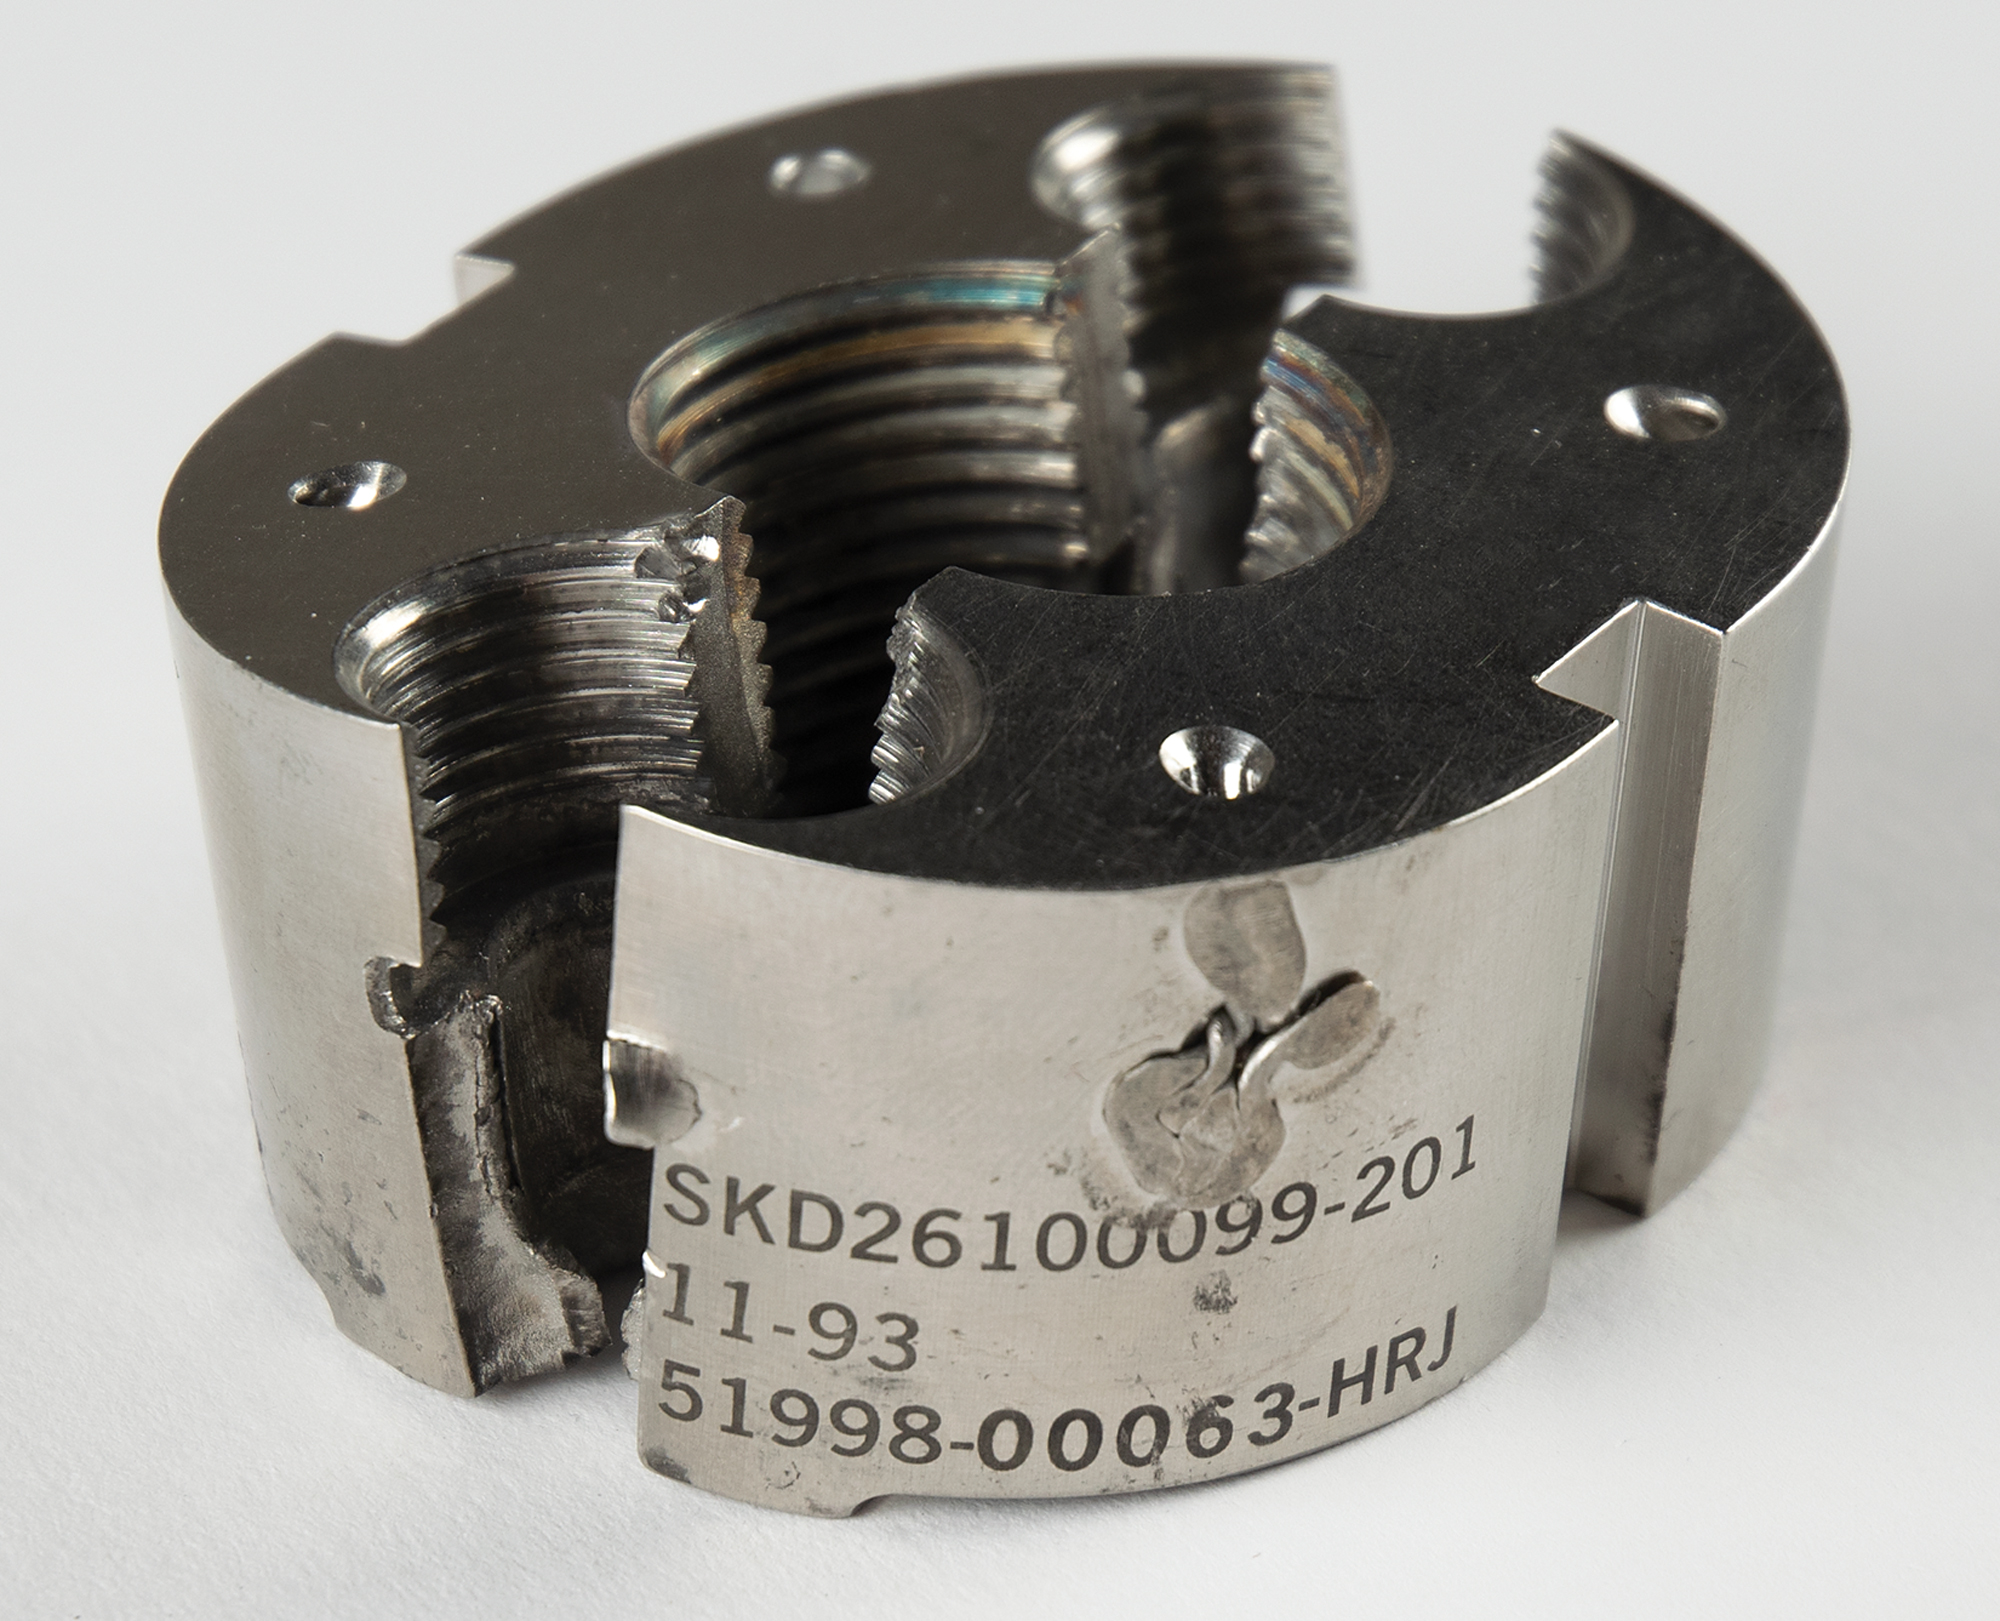
\includegraphics[width=0.4\textwidth]{figures/3454621_1.jpg}
    \caption{Boulon explosif ayant été utilisé sur les navettes spatiales américaines}
\end{figure}

\subsubsubsection{Non-pyrotechnique (mécanique / actionneurs)}

Les mécanismes non-pyrotechniques reposent sur des actionneurs, ressorts, latches ou systèmes cinématiques qui libèrent les
connections sans explosion. Ces solutions sont souvent utilisées dans des contextes où l’usage d’explosifs est indésirable ou
interdit.\\

\begin{itemize}
    \item \textbf{Mode d’activation :} Un système mécanique (servo-moteur, ressort à compression, actionneur linéaire) pousse ou
    désaccouple les éléments de fixation, libérant la contrainte.
    \item \textbf{Efforts mobilisés :} Forces généralement plus faibles et contrôlées, avec possibilité de modulation progressive
    des mouvements.
    \item \textbf{Avantages :} Moindre choc mécanique, possibilité de réversibilité ou de test au sol répétable.
    \item \textbf{Inconvénients :} Complexité mécanique accrue, risques d’enrayement ou d’erreur de synchronisation, besoins de
    commande et d’alimentation électrique supplémentaires.\\
\end{itemize}

Ce type de mécanisme est illustré par des solutions développées sur des projets étudiants ou petits lanceurs, où des serrures
mécaniques à bande associées à des actuateurs à fil résistif permettent un désaccouplement contrôlé avec faible impact
structurel \cite{EPFL_Separation}.

\subsubsection{Stratégies de séparation d’étages}

Au-delà du type de mécanisme utilisé pour rompre la liaison mécanique, la séquence de séparation joue un rôle majeur dans la
dynamique du vol. Deux stratégies opposées sont employées selon les architectures : la séparation à froid et à chaud
\cite{Multistage_Rocket}.

\subsubsubsection{Séparation à froid}

Dans une stratégie de séparation à froid, la séparation mécanique est effectuée avant l’allumage du moteur de l’étage supérieur.
L’étage inférieur termine sa combustion, se détache, puis le moteur du deuxième étage est mis en route après un court intervalle.

\begin{itemize}
    \item \textbf{Mode d'activations :} Séparation mécanique puis intervalle libre puis allumage du moteur supérieur.
    \item \textbf{Efforts mobilisés :} Efforts d’éloignement donnés par les dispositifs de séparation, puis poussée indépendante
    du moteur supérieur.
    \item \textbf{Avantages :} Isolation claire des phases de séparation et d’allumage, moins d’interactions thermiques ou
    mécaniques entre étages.
    \item \textbf{Inconvénients :} Nécessite un effort de séparation élevé pour assurer un éloignement suffisant avant l’allumage, ce qui
    peut imposer des dispositifs plus robustes et lourds.\\
\end{itemize}

Ce schéma est traditionnellement utilisé dans de nombreuses architectures occidentales (ex. Atlas, Titan, Saturn) où la finalité
est une séparation nette avant l’allumage moteur \cite{Multistage_Rocket}.

\subsubsubsection{Séparation à chaud}

Dans la séparation à chaud, le moteur de l’étage supérieur est allumé avant ou au moment de la séparation mécanique. Cette
approche utilise la poussée du moteur supérieur pour aider à éloigner les étages.\\

\begin{itemize}
    \item \textbf{Mode d'activations :} Allumage du moteur supérieur avant la séparation mécanique complète.
    \item \textbf{Efforts mobilisés :} Poussée continue transmise, ainsi qu’efforts de séparation mécanique.
    \item \textbf{Avantages :} Peut simplifier certaines interfaces mécaniques et augmenter l’impulsion disponible.
    \item \textbf{Inconvénients :} Interactions thermiques et dynamiques complexes entre jets moteurs et structure résiduelle ;
    demande une chonologie précise de la séquence de séparation.\\
\end{itemize}

Ce mode est caractéristique des architectures russes telles que Soyouz et Proton, et était prévu pour des programmes comme celui
de la fusée lunaire soviétque N1 \cite{Multistage_Rocket}. Elle est également la solution utiliser dans certains projets tel
que le lanceur Starship de SpaceX.

\begin{figure}[ht]
    \centering
    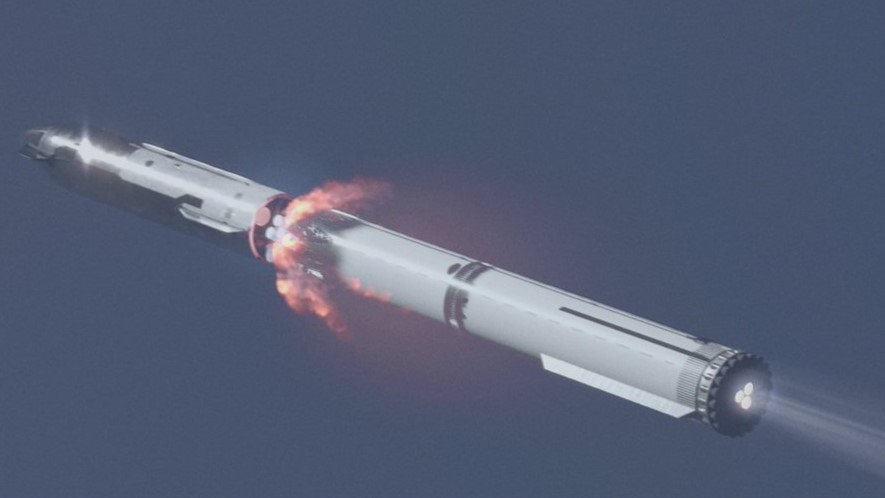
\includegraphics[width=0.9\textwidth]{figures/F3wgivuWkAAI7dq.jpg}
    \caption{Séparation à chaud du lanceur Starship de SpaceX}
\end{figure}

\subsubsection{Séparation à chaud sans connexion mécanique}

Parmi les diverses stratégies de séparation d'étage utilisées dans les lanceurs multi-étages, une approche particulière sans
connexion mécanique entre les étages a émergé dans certains contextes expérimentaux, notamment dans plusieurs projets américains
de petite échelle. Dans ce mode, les étages sont simplement empilés sans fixation structurelle rigide : l’étage supérieur repose
sur l’étage inférieur sans liaison mécanique formelle, et la séparation est obtenue uniquement par l’allumage du moteur du second
étage \cite{Whitman_2025_HotStagingModule}.L’absence de dispositifs de séparation classiques (boulons pyrotechniques, actionneurs,
ressorts) réduit drastiquement le nombre de sous-systèmes nécessaires pour réaliser la séparation, facilitant une simplification
mécanique attractive pour des équipes à ressources limitées.\\

L’effort mobilisé est essentiellement la poussée continue du moteur supérieur, qui doit non seulement accélérer le haut de la
fusée vers l’avant, mais aussi fournir l’impulsion relative nécessaire pour éloigner l’étage inférieur. Contrairement aux
mécanismes pyrotechniques ou mécaniques classiques, il n’y a pas de force transmise par une rupture contrôlée d’une liaison
structurelle : toute la dynamique de séparation dépend du flux de poussée du second étage.\\

Cette approche présente plusieurs avantages potentiels pour les lanceurs expérimentaux :
\begin{itemize}
    \item \textbf{Simplicité apparente du système de séparation :} l’élimination des éléments de séparation active (boulons,
    mécanismes, ressorts) réduit le nombre de pièces et donc les points de défaillance potentiels. Cela peut alléger la charge de
    conception et de fabrication dans un cadre associatif ou éducatif.
    \item \textbf{Réduction de la masse et de la complexité mécanique :} sans dispositifs de séparation dédiés, les interfaces
    entre étages restent minimalistes.
    \item \textbf{Facilité de test et d’intégration :} l’absence de mécanismes complexes permet des essais plus simples au sol,
    sans nécessiter de procédures de sécurité lourdes liées aux explosifs ou aux systèmes mécaniques sous tension.\\
\end{itemize}

Cependant, l’absence de liaison mécanique structurée entre les étages introduit des défis significatifs, qui sont particulièrement
critiques sur des véhicules à petite échelle :

\begin{itemize}
    \item \textbf{Absence de continuité structurelle :} sans fixation rigide, l’étage supérieur et l’étage inférieur ne partagent
    pas de lien structurel capable d’amortir ou de répartir les charges dynamiques. Cela implique que toute perturbation
    extérieure, vent latéral, irrégularité du vol ou micro-oscillation, peut provoquer une oscillation non atténuée du haut de
    l’étage avant séparation, ce qui peut affecter la trajectoire globale. À la différence des systèmes avec liaisons
    structurelles, où les étages restent couplés mécaniquement jusqu’à l’événement de séparation proprement dit, l’absence de
    cette contrainte rend le haut de la fusée plus sensible aux perturbations.
    \item \textbf{Contraintes sur la stabilité de trajectoire :} ce mode de staging exige une trajectoire dynamique parfaitement
    stabilisée avant l’allumage du moteur supérieur. La moindre erreur de centrage aerodynamique ou déséquilibre du véhicule peut
    se manifester sous forme de mouvement de tangage, lacet ou de roulis non atténués, car il n’existe pas de structure commune
    pour résorber ces effets.\\
\end{itemize}

Des travaux académiques récents illustrent l’intérêt de concevoir des modules de séparation chaude pour des fusées à deux étages
sans mécanismes de séparation traditionnels. Par exemple, une équipe universitaire a conçu un \textit{\og{}Hot Staging
Module\fg{}} en explorant des outils de simulation numérique (CFD) pour valider cette approche
\cite{Whitman_2025_HotStagingModule}. Ces projets soulignent l’intérêt de réduire le nombre de modes de défaillance liés aux
mécanismes classiques, mais insistent sur la nécessité d’une analyse dynamique approfondie du système de staging pour assurer la
stabilité et prédictibilité du comportement en vol.

\newpage

\subsubsection{Avantages et limitations des principaux modes et stratégies de séparation}

\begin{table}[h!]
\centering
\renewcommand{\arraystretch}{1.3}
\begin{tabular}{|p{2cm}|p{2.25cm}|p{2.25cm}|p{3.5cm}|p{3.5cm}|}
\hline
\textbf{Mode / \newline stratégie} &
\textbf{Mode d’activation} &
\textbf{Efforts mobilisés} &
\textbf{Avantages principaux} &
\textbf{Limitations principales} \\
\hline

Séparation pyrotechnique &
Détonation contrôlée &
Impulsion mécanique brusque &
Fiabilité élevée, séparation rapide, technologie éprouvée &
Chocs mécaniques importants, irréversibilité, contraintes réglementaires liées aux explosifs \\
\hline

Séparation mécanique &
Actionneur, ressort ou système cinématique &
Efforts progressifs et contrôlés &
Réduction des chocs, testabilité au sol, absence d’explosifs &
Complexité mécanique accrue, risques d’enrayement, besoins en énergie et en commande \\
\hline

Séparation à froid &
Séparation mécanique puis allumage moteur &
Efforts de séparation dédiés uniquement &
Découplage clair entre séparation et propulsion, interactions limitées &
Effort de séparation plus élevé requis, présence possible de systèmes auxiliaires (ullage) \\
\hline

Séparation à chaud &
Allumage moteur avant ou pendant la séparation &
Poussée moteur combinée à la séparation mécanique &
Réduction de l’effort de séparation, simplification partielle des sous-systèmes &
Contraintes thermiques et dynamiques, séquence de séparation critique \\
\hline

Séparation chaude sans connexion mécanique &
Allumage moteur du second étage uniquement &
Poussée moteur seule &
Simplicité structurelle maximale, masse réduite, peu de sous-systèmes &
Forte exigence de stabilité, sensibilité aux perturbations externes, domaine d’emploi restreint \\
\hline

\end{tabular}
\caption{Comparaison des principaux modes et stratégies de séparation d’étages}
\label{tab:separation_modes}
\end{table}

L’analyse comparative des principaux modes de séparation met en évidence l’absence de solution universelle, chaque approche
reposant sur un compromis entre simplicité mécanique, maîtrise dynamique et complexité opérationnelle.\\

Les systèmes pyrotechniques, largement éprouvés dans le domaine spatial industriel, offrent une séparation rapide et fiable, mais
au prix de chocs mécaniques élevés, d’une irréversibilité totale et de contraintes réglementaires incompatibles avec de nombreux
projets expérimentaux. À l’inverse, les solutions non-pyrotechniques réduisent les niveaux de choc et améliorent la testabilité,
mais introduisent une complexité mécanique et fonctionnelle qui peut devenir pénalisante dans des architectures légères et à
ressources limitées.\\

Du point de vue des stratégies de staging, la séparation à froid privilégie une séquence clairement découplée entre séparation et
propulsion, au prix d’efforts de séparation dédiés. La séparation à chaud, en exploitant directement la poussée du moteur
supérieur, permet de réduire ces efforts mais impose une gestion fine des interactions thermiques et dynamiques au moment de la
séparation.\\

Enfin, le hot staging sans connexion mécanique, observé dans certains projets expérimentaux, illustre une recherche de simplicité
extrême en supprimant tout dispositif de séparation dédié. Cette approche transfère toutefois l’essentiel des contraintes vers la
stabilité aérodynamique et inertielle du véhicule, rendant le système particulièrement sensible aux perturbations extérieures et
limitant fortement son domaine d’application.\\

Dans le contexte des lanceurs expérimentaux et des fusées sondes, ces constats soulignent que la problématique de la séparation
d’étages ne se résume pas à un choix technologique isolé, mais relève d’un équilibre global entre architecture, dynamique du vol
et contraintes opérationnelles. Cette analyse justifie l’exploration de solutions intermédiaires, capables de générer un effort
de séparation maîtrisé sans recourir à des dispositifs pyrotechniques ni à des mécanismes complexes, tout en limitant les
exigences imposées à la stabilité du véhicule.


\subsubsection{Principe de la solution étudiée : séparation assistée par aérofreinage}

L’état de l’art met en évidence une grande diversité de systèmes de séparation d’étages, reposant sur des compromis différents
entre fiabilité, complexité mécanique, maîtrise des efforts transmis et exigences sur la stabilité du véhicule. Aucune de ces
solutions ne s’impose comme universelle dans le cadre des lanceurs expérimentaux, où les contraintes de simplicité, de sûreté et
de moyens d’essai limités occupent une place centrale.\\

Dans ce contexte, le présent travail propose d’explorer une approche alternative, fondée sur l’exploitation des efforts
aérodynamiques disponibles en phase atmosphérique. Le principe de la séparation assistée par aérofreinage consiste à provoquer
une augmentation volontaire de la traînée sur l’étage inférieur, au moyen de dispositifs aérodynamiques déployables, afin de
créer une décélération différentielle entre les deux étages. Cette dissymétrie d’efforts aérodynamiques génère un effort
longitudinal relatif qui contribue à initier l’éloignement des étages de manière progressive, sans recours à des charges
pyrotechniques ni à des mécanismes énergétiques dédiés.\\

Afin de permettre l’évaluation expérimentale de ce principe dans des conditions représentatives d’un lanceur expérimental, le
projet SP-02 repose sur la réalisation d’une fusée bi-étage spécifiquement conçue comme vecteur d’essai. L’architecture retenue
intègre des aérofreins destinés à générer l’effort de séparation étudié, tout en conservant une continuité structurelle contrôlée
entre les étages jusqu’à l’événement de séparation. Un dispositif mécanique à ressort, indépendant du mécanisme aérodynamique et
activé de manière décalée, est également intégré afin de garantir la séparation effective du véhicule, y compris en cas
d’efficacité insuffisante du phénomène d’aérofreinage.\\

La compréhension et l’analyse de ce principe de séparation reposent directement sur les caractéristiques géométriques,
structurelles et aérodynamiques du vecteur expérimental. La section suivante est ainsi consacrée à la présentation du lanceur
SP-02, de sa philosophie de conception et de son rôle en tant que support d’expérimentation pour l’étude de la séparation
d’étages assistée par aérofreinage.

\newpage
